
\documentclass{beamer}
\usepackage{HECbeamer}
\usepackage{icomma}

\title[\color{white}{MATH 60604 \S~5d - Équicorrélation}]{\texorpdfstring{MATH 60604 \\Modélisation statistique \\ \S~5d - Équicorrélation}{MATH 60604 \\Modélisation statistique \\ \S~5d - Équicorrélation}}
\author{}
\institute{HEC Montréal\\
Département de sciences de la décision}
\date{} 

\begin{document}
\frame{\titlepage}

\begin{frame}
\frametitle{Covariance du modèle d'équicorrélation}
\bi
\item Supposons que les
observations d'un même groupe sont interchangeables. Plus précisément, 
supposons que la corrélation (conditionnelle aux variables explicatives) entre
deux observations $Y$ d'un groupe est toujours la même et que la variance (conditionnelle) de $Y$ est constante.
\item S'il y a cinq observations dans le groupe $i$ , la matrice de covariance est
{\small \[
\bs{\Sigma}_i=
  \begin{pmatrix}
    \sigma^2+\tau & \tau & \tau & \tau & \tau\\
    \tau & \sigma^2+\tau & \tau& \tau & \tau\\
    \tau & \tau & \sigma^2+\tau & \tau & \tau\\
    \tau & \tau & \tau & \sigma^2+\tau & \tau\\
    \tau & \tau & \tau & \tau & \sigma^2+\tau
  \end{pmatrix}.
\]
}
\item Cette paramétrisation est utilisée par \SASlang{}. 
\item Il est important de comprendre que la covariance
(conditionnelle) entre deux observations quelconques est $\tau$ et que la
variance (conditionnelle) de chaque observation est $\sigma^2+\tau$.
\ei
\end{frame}

\begin{frame}
\frametitle{Corrélation du modèle d'équicorrélation}
La matrice de corrélation correspondante du modèle d'équicorrélation est
\[
\mathbf{R}_i=
  \begin{pmatrix}
   1 & \rho & \rho & \rho & \rho\\
    \rho &1 & \rho & \rho & \rho\\
   \rho & \rho & 1 &\rho & \rho\\
   \rho & \rho & \rho & 1 &\rho\\
   \rho & \rho & \rho & \rho &1
  \end{pmatrix}, 
\]
où $\rho=\tau/(\sigma^2+\tau)$.
\bi
\item La corrélation (conditionnelle) entre deux observations
au sein d'un même groupe est toujours $\rho$. 
% \item Si on suppose que cette structure de
% covariance (corrélation) est la même dans tous les groupes, elle dépend alors
% de seulement deux paramètres $\sigma^2$ et $\tau$, qui seront estimés. 
Cette structure
de covariance porte le nom \alert{d'équicorrélation} (\textit{compound symmetry} en anglais) et dépend de deux paramètres $\sigma^2$ et $\tau$.
\ei
\end{frame}

 \begin{frame}[fragile]
\frametitle{Procédure \texttt{mixed} pour les données corrélées}

\begin{tcolorbox}[colback=white, colframe=hecblue, title=Code SAS pour ajuster le modèle d'équicorrélation]
\begin{verbatim}
/* Créer une copie de t */
data vengeance; 
set modstat.vengeance; 
tcat=t; 
run;

proc mixed data=vengeance method=reml; 
class id tcat; 
model vengeance = sexe age vc wom t / solution; 
repeated tcat / subject=id type=cs r=1 rcorr=1; 
run;
\end{verbatim}
\end{tcolorbox}
\end{frame}
% \begin{frame}
% \frametitle{Syntaxe de \texttt{proc mixed}} 
% \begin{center}
%  \includegraphics[width = 0.9\linewidth]{img/c5/06-correlated-proc_mixed_syntax.pdf}
%  \end{center}
% \end{frame}
\begin{frame}
\frametitle{Spécification de la structure de dépendance dans \texttt{proc mixed}}
La commande \texttt{\textbf{repeated}} permet de définir la structure de dépendance des données.
\bi
\item Le premier argument de la commande \code{\textbf{repeated}} spécifie l'ordre des observations au sein du groupe (utile pour les données longitudinales). Cette variable doit être catégorielle (déclarée via \code{\textbf{class}}).
\item L'option  \code{\textbf{subject}} définit la variable qui identifie les groupes d'observations. 
\item L'option \code{\textbf{type}} spécifie le modèle de covariance intra-groupe. 
\item L'option \code{r=1} (\code{rcorr=1}) demande que l'estimation de la matrice de covariance (corrélation) de la personne 1 soit présentée dans la sortie.
\ei
{\footnotesize 
Comme nous voulons aussi utiliser la variable \code{t} dans le modèle en tant que variable continue, nous avons créé une autre variable \code{t} (\code{tcat} ici), afin de pouvoir l'utiliser comme argument de  \code{\textbf{repeated}}. 

}
\end{frame}
% 
% 
% 
%  \begin{frame}[fragile]
% \frametitle{Exemple: explication du code SAS}
% \bi
% \item L'argument premier de  \code{\textbf{repeated}} est la variable \code{tcat} que nous venons de créer. C'est la variable qui sert à dire dans quel ordre sont les observations à l'intérieur d'un groupe. Il faut absolument que ça soit une variable définie dans \code{\textbf{class}}. 
% \item Comme nous voulons aussi utiliser la variable \code{t} dans le modèle en tant que variable continue, cela explique pourquoi nous avons créé une autre variable \code{t} (\code{tcat} ici), afin de pouvoir l'utiliser comme argument de  \code{\textbf{repeated}}. 
% \item L'option  \code{\textbf{type}} donne la structure de covariance voulue. Ici, c'est la structure  \code{cs}, pour ``compound symmetry''. 
% 
% \ei
% \end{frame}


\begin{frame}[fragile]
\frametitle{Disgression technique}
\bi
\item Comme la structure utilisée est \code{cs}, nous n'aurions pas eu besoin de donner l'argument premier \texttt{tcat} à  \code{\textbf{repeated}}  car cette structure n'utilise pas l'ordre des observations à l'intérieur d'un groupe. 
% \item En effet, la structure d'équicorrélation suppose que la corrélation (conditionnelle) entre deux observations d'un groupe est la même peu importe où ces observations se trouvent à l'intérieur du groupe. 
\item L'ordre est en revanche important pour d'autres types de structure, comme le modèle autorégressif. Ça ne fait pas de tort de conserver l'information.
\ei
\end{frame}

\begin{frame}[fragile]
\frametitle{Spécification du modèle}
\begin{center}
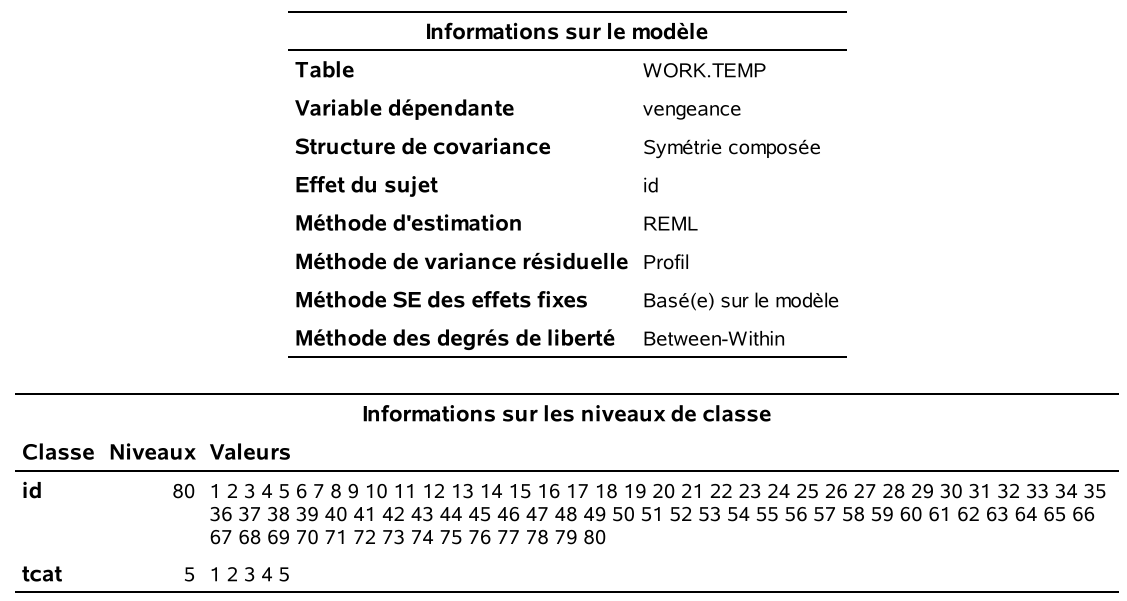
\includegraphics[width = \linewidth]{img/c5/diapos6-e06}
\end{center}
\end{frame}
\begin{frame}[fragile]
\frametitle{Matrices de covariance et de corrélation pour l'individu $1$}
\begin{center}
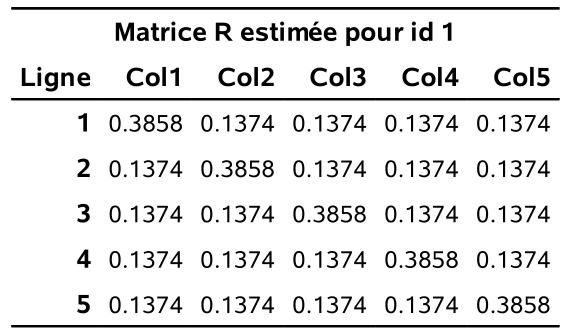
\includegraphics[width = 0.45\linewidth]{img/c5/diapos6-e07a}
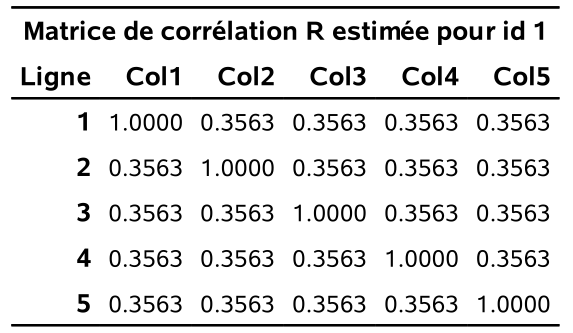
\includegraphics[width = 0.45\linewidth]{img/c5/diapos6-e07b}
\end{center}
Avec la structure d'équicorrélation, la corrélation est la même pour toutes les mesures répétées de l'individu $1$.

\end{frame}
% \begin{frame}[fragile]
% \frametitle{Exemple vengeance: sortie SAS}
% \textbf{Spécification du modèle}
% \begin{center}
% \includegraphics[scale=0.35]{Figures/long14.pdf}
% \includegraphics[scale=0.35]{Figures/long15.pdf}
% \end{center}
% \bi
% \item Dans le tableau de droite (haut), $X$ représente la matrice des effets fixes et $Z$ la matrice des effets aléatoires. 
% \item Ici, on n'a pas d'effet aléatoires
% \ei
% \end{frame}
% 
% \begin{frame}[fragile]
% \frametitle{Exemple vengeance: sortie SAS}
% \textbf{Matrice de covariance et de corrélation pour l'individu 1:}
% \begin{center}
% \includegraphics[scale=0.5]{Figures/long16_1.pdf}
% \includegraphics[scale=0.5]{Figures/long17_1.pdf}
% \end{center}
% \bi
% \item On voit bien que la correlation est la même pour toutes les observations à l'intérieur du sujet 1
% \item C'est bien ce qu'on avait demandé avec la structure de corrélationCS
% \ei
% \end{frame}

\begin{frame}[fragile]
\frametitle{Paramètres de la structure de covariance}
\begin{center}
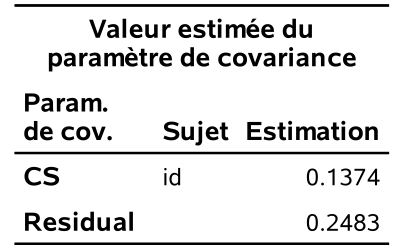
\includegraphics[width = 0.4\linewidth]{img/c5/diapos6-e08}
\end{center}
\bi
\item La covariance intra-groupe du modèle d'équicorrélation est paramétrisé avec
\bi
\item $\Va{Y_{ij}}=\sigma^2+\tau$;
\item $\Co{Y_{ij}, Y_{ij'}}=\tau$.
\ei
\item L'estimé de la covariance conditionnelle entre observations pour une personne donnée est $\hat{\tau}=0.137$.
\item L'estimé de la covariance conditionnelle d'une observation est $\hat{\tau}+ \hat{\sigma}^2= 0.386$.
\ei
\end{frame}

\begin{frame}[fragile]
\frametitle{Exemple: structure de corrélation}
\bi

\item Par conséquent, l'estimation de la corrélation (conditionnelle) entre deux
observations d'une même personne (corrélation intra-classe) est donc :
\begin{align*}
\hat{\rho}=\frac{\hat{\tau}}{\hat{\tau}+\hat{\sigma}^2}=\frac{0.137}{0.137+0.248}=0.356.
\end{align*}
\item On peut retrouver ces valeurs dans les matrices de covariance et de
corrélation fournies pour la première personne.
\item \textbf{Vous devez être en mesure de reconstruire la corrélation sur la base de la sortie (d'où l'importance de comprendre la formule).}
\ei
% \item 
% \item  Toujours dans le tableau ``Covariance Parameter Estimates'', on voit que le
% paramètre $\tau$ est significativement différent de 0. 
% \item \alert{Il y donc bel et bien une corrélation (covariance) non-nulle entre deux
% observations d'une même personne, même après avoir tenu compte des effets
% des variables explicatives. De plus, cette corrélation est positive.}
% \ei
\end{frame}



\begin{frame}[fragile]
\frametitle{Test du rapport de vraisemblance pour le paramètre $\tau$}

\begin{center}
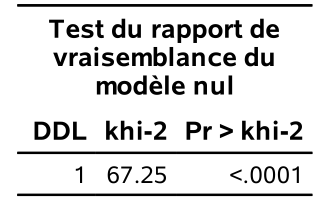
\includegraphics[width = 0.35\linewidth]{img/c5/diapos6-e09}
\end{center}
\bi
\item 
On peut tester l'hypothèse $\Hy_0:\tau=0$ versus l'alternative $\Hy_1: \tau \neq 0$ à l'aide d'un \textbf{test du rapport de vraisemblance}.
\item Le tableau ci-dessus donne la statistique de test pour $\Hy_0: \tau=0$, qui correspond au modèle de covariance $\sigma^2\mathbf{I}$ du modèle de régression linéaire classique (modèle réduit), ajusté par REML.
\item On conclut que le modèle réduit sans corrélation n'est pas une \textbf{simplification adéquate} du modèle complet  avec une structure d'équicorrélation.
\item \textbf{Le test du rapport de vraisemblance produit par \SASlang{}{} compare toujours le modèle ajusté au modèle linéaire homoscédastique sans corrélation.}
\ei
% \item We can do the test manually: the linear model without any structure had $-2\ell_{\textrm{reml}}(\hat{\bs{\theta}}_0)=776.7.$
\end{frame}


\begin{frame}[fragile]
\frametitle{Test du rapport de vraisemblance à la mitaine}
\begin{center}
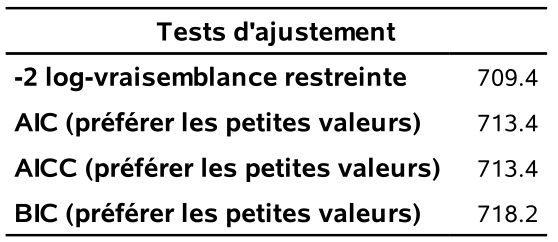
\includegraphics[width = 0.35\linewidth]{img/c5/diapos6-e10}
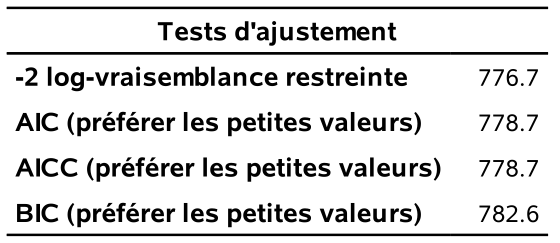
\includegraphics[width = 0.35\linewidth]{img/c5/diapos6-e11}
\end{center}
\bi 
\item On peut obtenir la valeur de la statistique de test manuellement en comparant les valeurs de la vraisemblance REML des deux modèles, ici $-2\ell_{\textrm{reml}}(\hat{\bs{\theta}}_0)=776.7$ et $-2\ell_{\textrm{reml}}(\hat{\bs{\theta}})=709.4$. La statistique est $67.3$. 
\bi
\item {\footnotesize C'est la même valeur que dans le tableau, à arrondi près. }
\ei 
\item La distribution nulle du test de rapport de vraisemblance est  $\chi^2_1$ (pourquoi?).
\item On peut comparer la valeur du test au quantile $95\%$ de la loi $\chi^2_1$, $3.84$. Puisque la valeur de la statistique est supérieure à $3.84$, on rejette $\Hy_0$ à niveau $\alpha=0.05$.
\ei
\end{frame}
\begin{frame}[fragile]
\frametitle{Estimés des paramètres de moyenne}
\begin{center}
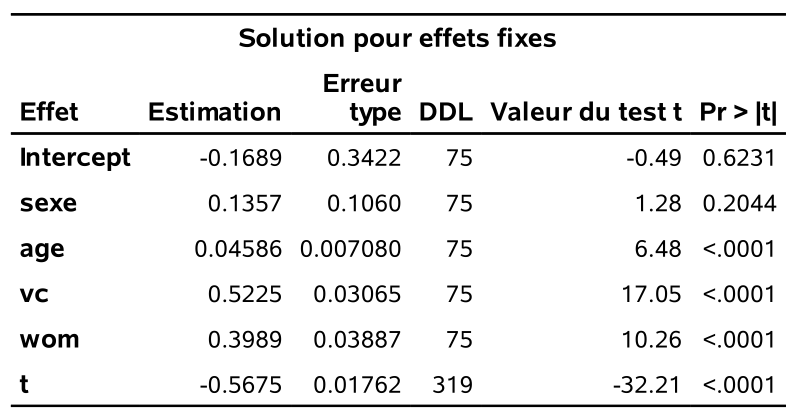
\includegraphics[width = 0.7\linewidth]{img/c5/diapos6-e12}
\end{center}
Le désir de vengeance décroît avec le temps, une fois qu'on contrôle pour l'effet des autres variables.
\end{frame}

\begin{frame}[fragile]
\frametitle{Estimés des coefficients}
\bi
\item Le modèle ajusté est toujours un modèle linéaire, 
\begin{align*}
\widehat{\code{vengeance}}=&-0.169 + 0.136 \code{sexe} + 0.0459 \code{age} + 0.523 \code{vc}\\
 & \qquad + 0.399 \code{wom} -0.568 \code{t}.
\end{align*}
\item  Les estimés des paramètres $\bs{\beta}$ sont exactement les mêmes que ceux du modèle de régression linéaire ordinaire.
\item C'est vrai seulement pour le cas spécial  du modèle d'équicorrélation avec le même nombre d'observations dans chaque groupe.
\item En général, cependant, les estimés d'autres modèles ne seront pas très différents de ceux du modèle linéaire ordinaire s'ils ont les mêmes régresseurs, mais des structures de covariance différentes.
\ei
\end{frame}




\begin{frame}[fragile]
\frametitle{Comparaison des coefficients du modèle}

\begin{center}
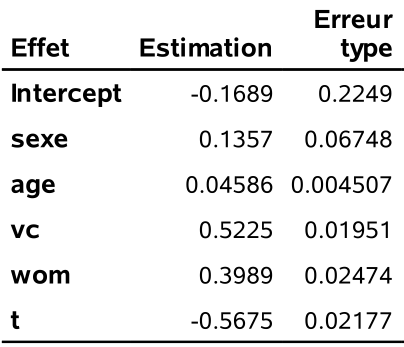
\includegraphics[width = 0.35\linewidth]{img/c5/diapos6-e13}
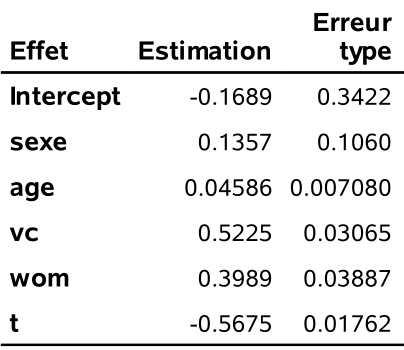
\includegraphics[width = 0.35\linewidth]{img/c5/diapos6-e14}
\end{center}
{\small
\bi
\item La précision des estimés $\hat{\bs{\beta}}$ change (à gauche modèle linéaire ordinaire, à droite le modèle avec équicorrélation).
\item Les erreurs-types des paramètres sont plus grandes dans le modèle d'équicorrélation. Les conclusions sur la significativité des paramètres ne changent pas, hormis pour la variable \code{sexe} qui n'est plus significative.
\item La corrélation intra-groupe rend les observations partiellement redondantes: on a moins d'information qu'avec un échantillon de même taille avec uniquement des données indépendantes, donc les estimés des paramètres sont moins précis.
\ei
}
\end{frame}




\end{document}
